% Moebius Traces: Depth from Motion along Curved Paths
% VISGRAF Lab technical note. 19 November 2026.
% Build: pdflatex twice, in this folder (or Overleaf with this file as the main document).
% Figures in figs/ come from the records of visgraf/deep-motion (figs/SOURCES.md).
\documentclass[11pt,a4paper]{article}

\usepackage[T1]{fontenc}
\usepackage[utf8]{inputenc}
\IfFileExists{lmodern.sty}{\usepackage{lmodern}\usepackage{microtype}}{\usepackage[expansion=false]{microtype}}
\usepackage[a4paper,top=2.5cm,bottom=2.6cm,left=2.6cm,right=2.6cm]{geometry}
\usepackage{textcomp}
\usepackage{amsmath,amssymb}
\usepackage{booktabs}
\usepackage{tabularx}
\usepackage{array}
\usepackage{xcolor}
\usepackage{enumitem}
\usepackage{graphicx}
\usepackage[font=small,labelfont=bf]{caption}
\usepackage{placeins}
\usepackage[hidelinks]{hyperref}
\hypersetup{colorlinks=true,linkcolor=black!70!blue,citecolor=black!70!blue,urlcolor=black!70!blue,
  pdftitle={Moebius Traces: Depth from Motion along Curved Paths},
  pdfauthor={Luiz Velho, with Claude (Anthropic)},
  pdfsubject={VISGRAF technical note, 19 November 2026}}
% figures resolve whether the compile runs in this folder or at the repository's root
\graphicspath{{figs/}{moebius-traces/figs/}}

% ---------------------------------------------------------------- VISGRAF cover
\IfFileExists{techrep-ic.sty}{%
  \usepackage{techrep-ic}%
  \newcommand{\MakeVisgrafCover}{%
    \TRNumber{17}   % <-- placeholder: set the report number (printed as TR-26-XX)
    \TRYear{26}
    \TRMonth{11}
    \TRAuthor{Luiz Velho, Claude}
    \TRTitle{M\"obius Traces:\\Depth from Motion along Curved Paths}
    \TRMakeCover}%
}{\newcommand{\MakeVisgrafCover}{}}

% ---------------------------------------------------------------- helpers
\newcommand{\code}[1]{\texttt{\small #1}}
\newcommand{\cell}{\raggedright\arraybackslash}
\newcolumntype{L}{>{\cell}X}
\setlist{itemsep=2pt,topsep=4pt}
\renewcommand{\arraystretch}{1.15}
\setlength{\emergencystretch}{1.5em}
\renewcommand{\topfraction}{0.9}\renewcommand{\bottomfraction}{0.6}\renewcommand{\textfraction}{0.08}\renewcommand{\floatpagefraction}{0.8}
\newcommand{\src}[1]{\textsuperscript{\,#1}}
\newcommand{\WS}{\src{W}}   % measured by Claude Code on the workstation
\newcommand{\SB}{\src{S}}   % measured in the Chat sandbox
\newcommand{\mt}{M\"obius traces}

\title{\textbf{M\"obius Traces:\\Depth from Motion along Curved Paths}}
\author{Luiz Velho\\[2pt] \normalsize with Claude (Anthropic)\\[2pt]
  \normalsize VISGRAF Lab, IMPA}
\date{\normalsize Technical Note \textperiodcentered{} 19 November 2026\\[2pt]
  \normalsize Software and records: \url{https://github.com/visgraf/deep-motion}}

\begin{document}

\MakeVisgrafCover
\maketitle

\begin{abstract}
\noindent An eye that walks along a smooth path sees the world move in a way the path dictates. We choose image
coordinates in which that motion becomes a shift in time. For each piece of a path made of straight lines, circular arcs
and turns in place, a single number per scene point then predicts the point's whole trajectory across every image taken
along the piece: its distance $D$ to the path line, or its distance $\rho$ to the turn's axis. Depth estimation becomes a
one-dimensional search over that number. On the viewing sphere the structure is that of M\"obius transformations: a turn
of the eye is an elliptic M\"obius map and carries no depth; a translation moves every point along the orbits of a
hyperbolic M\"obius map, at a speed weighted by inverse range; an arc is their sum. We call the method \emph{\mt}. With a
perfect matcher (an oracle) on rendered scenes, it is calibrated (95\,\% intervals cover the truth 95\,\% of the time), it
fills the blind cone that a straight path leaves at its heading, and along a 4\,m tour of a classroom it measures 99\,\%
of the visible surface within $\pm10$\,\%. Matching real images along these traces is the open problem, and the next.
\end{abstract}

\noindent\small Numbers carry their source: \WS\ measured by Claude Code on the RTX~4090 workstation; \SB\ measured in
the Chat sandbox (CPU). Every number is in a record of the repository (\code{docs/plan.md} and
\code{docs/runs/}) or in the GitHub issue that reported it. All depth results in this note use an oracle (perfect
correspondences, with noise added); none uses real image matching.\normalsize

% ================================================================================================
\section{Why curved paths}\label{sec:why}

The previous note of this series~\cite{tr2} gave a foveated eye depth from its own forward motion. Under a straight
step every point slides along its radial line from the focus of expansion (FOE), and in the log-tangent coordinate
$q=\ln\tan e$ it moves by the same amount at a given axial depth. Matching a window of frames along that one axis
(multiple-baseline stereo~\cite{okutomi} in log-polar coordinates) gave usable depth over much of the periphery. A
demonstration tour of the Blender Classroom then joined straight runs with turns in place, because the method needs the
eye to look where it goes.

Real observers do not walk in polygons, and they do not always look where they go. The next experiments (foveal-motion
M6a) let the gaze turn away from the heading and the path curve. The geometry gained: with the epipole $10^\circ$ off the
fovea, an oracle found the whole fovea usable at 0.5\,px noise, against 0.004 on the straight dolly\SB. The matcher did
not: extended to the moving epipole it became more accurate (median error 0.61 to 0.30\,\%) but accepted less of the field
(0.34 to 0.27), because the motion now crossed its radial windows\SB. Rectifying about the epipole did not cure it.

The conclusion was to stop extending a representation built for one motion, and to build the representation on the
motion itself. This note collects that formulation and its first evaluation (repository \code{deep-motion}~\cite{dm}).

% ================================================================================================
\section{The idea in one picture}\label{sec:idea}

Pick coordinates in which the eye's motion acts as a \emph{shift in time}. Then a point's track through the image
sequence, its \emph{trace}, has a fixed shape, and points that share one number share one trace, only displaced in
time. That number is the depth we want. Guess it, and the guess predicts where the point must be in every image along
the path; the right guess is the one along which the images agree.

Figure~\ref{fig:traces-line} shows this for a straight path. Each ray is described by the plane through the path line
that contains it (angle $\omega$) and its angle $\psi$ from the heading. Translation never moves a point out of its plane,
and in the coordinate $u=\cot\psi$ a point at distance $D$ from the path line, after the eye has moved by $t$, is at
\begin{equation}\label{eq:line}
  u' = u - t/D .
\end{equation}
Every trace is a straight line of slope $-1/D$, and points with equal $D$ draw the same line, shifted in $t$. M4's
log-tangent coordinate is the same angle seen differently: $q=\ln\tan\psi$, in which a step shifts every point at axial
depth $z$ by $\ln(z/(z-t))$. Its traces curve and speed up as the point approaches, and its depth $z$ belongs to the
eye's current position: it changes at every step. $D$ does not change along the path. That is the difference that makes
the whole path, not a pair of frames, the unit of estimation.

\begin{figure}[t]
\centering
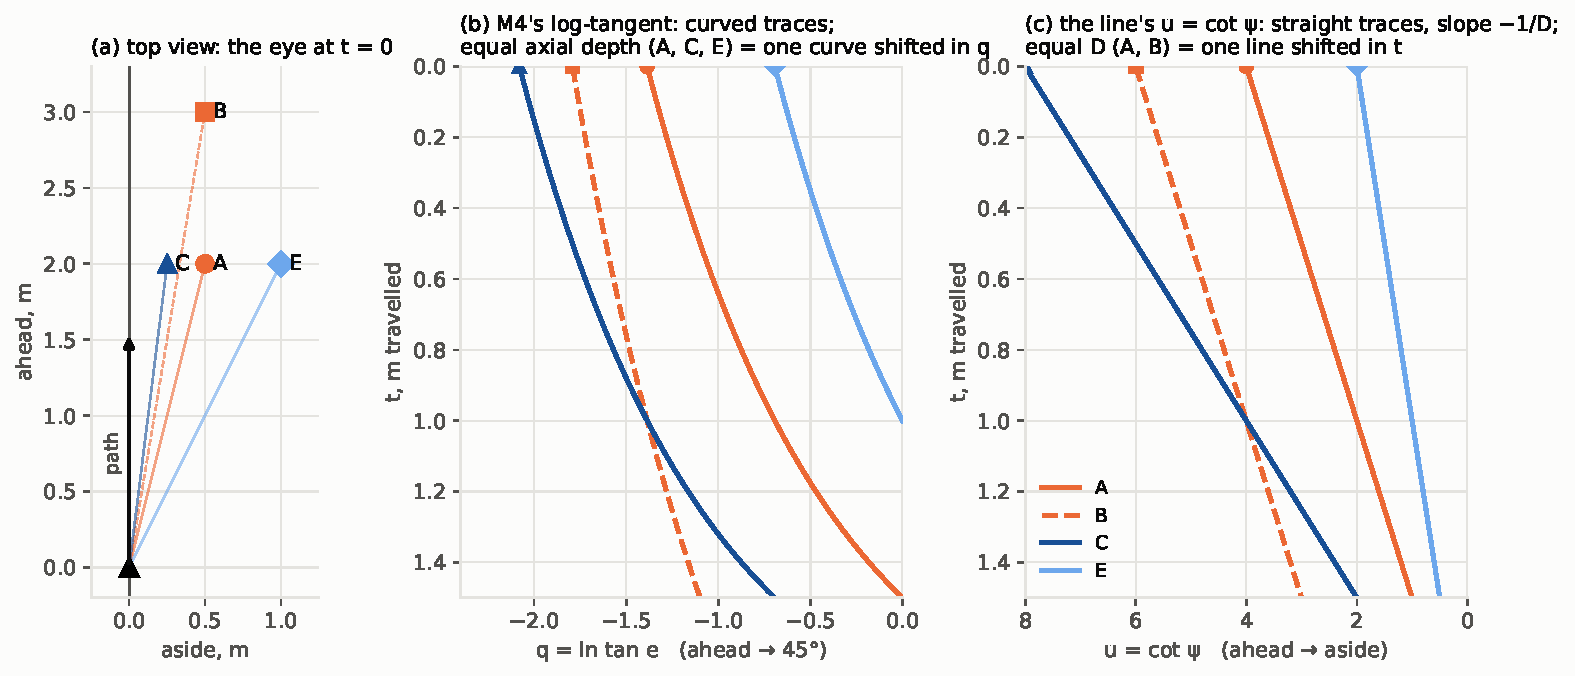
\includegraphics[width=\linewidth]{traces_line.pdf}
\caption{Four points beside a straight path (a), and their traces as the eye moves forward. (b) M4's log-tangent
$q=\ln\tan e$: the traces curve; points at the same axial depth (A, C, E, all 2\,m ahead) draw one curve shifted in $q$;
E leaves M4's $45^\circ$ field after half a metre. (c) The line's coordinate $u=\cot\psi$: every trace is straight with
slope $-1/D$; A and B, both 0.5\,m from the path line, draw one line shifted in $t$. Formulas only.}\label{fig:traces-line}
\end{figure}

% ================================================================================================
\section{Three primitives}\label{sec:primitives}

A path of constant curvature $\kappa=1/R$, travelled at constant speed with the head locked to its tangent, is the orbit
of a one-parameter group of rigid motions. One family gives three primitives, and a general path is approximated by a
sequence of them (Table~\ref{tab:primitives}).

\begin{table}[h]
\centering\small
\begin{tabularx}{\linewidth}{@{}l c L L L@{}}
\toprule
Primitive & $\kappa$ & Canonical coordinates & Depth invariant & Blind set \\
\midrule
Line & 0 & pencil of planes through the path line: $\omega$, $u=\cot\psi$ & $D$, distance to the path line & the path
line (the FOE and its opposite)\\
Arc & $1/R$ & concentric mosaics~\cite{shum}: slit angle $\beta$ to the tangent, arc angle $\theta$ & $\rho$, distance to the
turn axis & none for range\\
Pivot & $\infty$ & bearing relative to the heading & none & everything\\
\bottomrule
\end{tabularx}
\caption{The primitives. The arc's slit at angle $\beta$ is tangent to the circle of radius $R\cos\beta$; a point at radius
$\rho$ crosses it at $\theta_P-\delta$ with $\rho\cos\delta = R\cos\beta$ (two branches).}\label{tab:primitives}
\end{table}

Figure~\ref{fig:traces-primitives} follows the same four points under each primitive, as bearing against progress. Under
a turn in place every point's bearing changes by exactly the turn angle, whatever its distance: all traces are one
diagonal, and nothing in them depends on depth. Under a line the traces spread from the heading and close up behind. An
arc lies between: every trace leans like the turn's diagonal, and near points bend away from it. That bend is the
parallax, and it depends only on $\rho$. Points at equal $\rho$ draw the same curve, shifted in $\theta$.

Stage~2 of the project checked these closed forms against the exact projection of rendered geometry: the line's
equation~\eqref{eq:line} to $6.8\times10^{-14}$, the arc's crossing law to $3.1\times10^{-15}$ over 2{,}800 sightings, and
the time-shift symmetry to $7.8\times10^{-16}$, each with a control that fails (a path line turned $1^\circ$, a radius
2\,\% wrong, a point 5\,\% farther)\SB. With the gaze along the path, the line's coordinate reduces exactly to M4's:
$-\ln(u(s+t)/u(s))$ is M4's shift (to $3.6\times10^{-15}$)\SB.

What each representation estimates is drawn in Figure~\ref{fig:invariants}: M4's axial depth exists only within $45^\circ$
of the axis and only for the current position; $D$ and $\rho$ belong to the scene and the path, so every look along a
piece votes for the same number.

\begin{figure}[t]
\centering
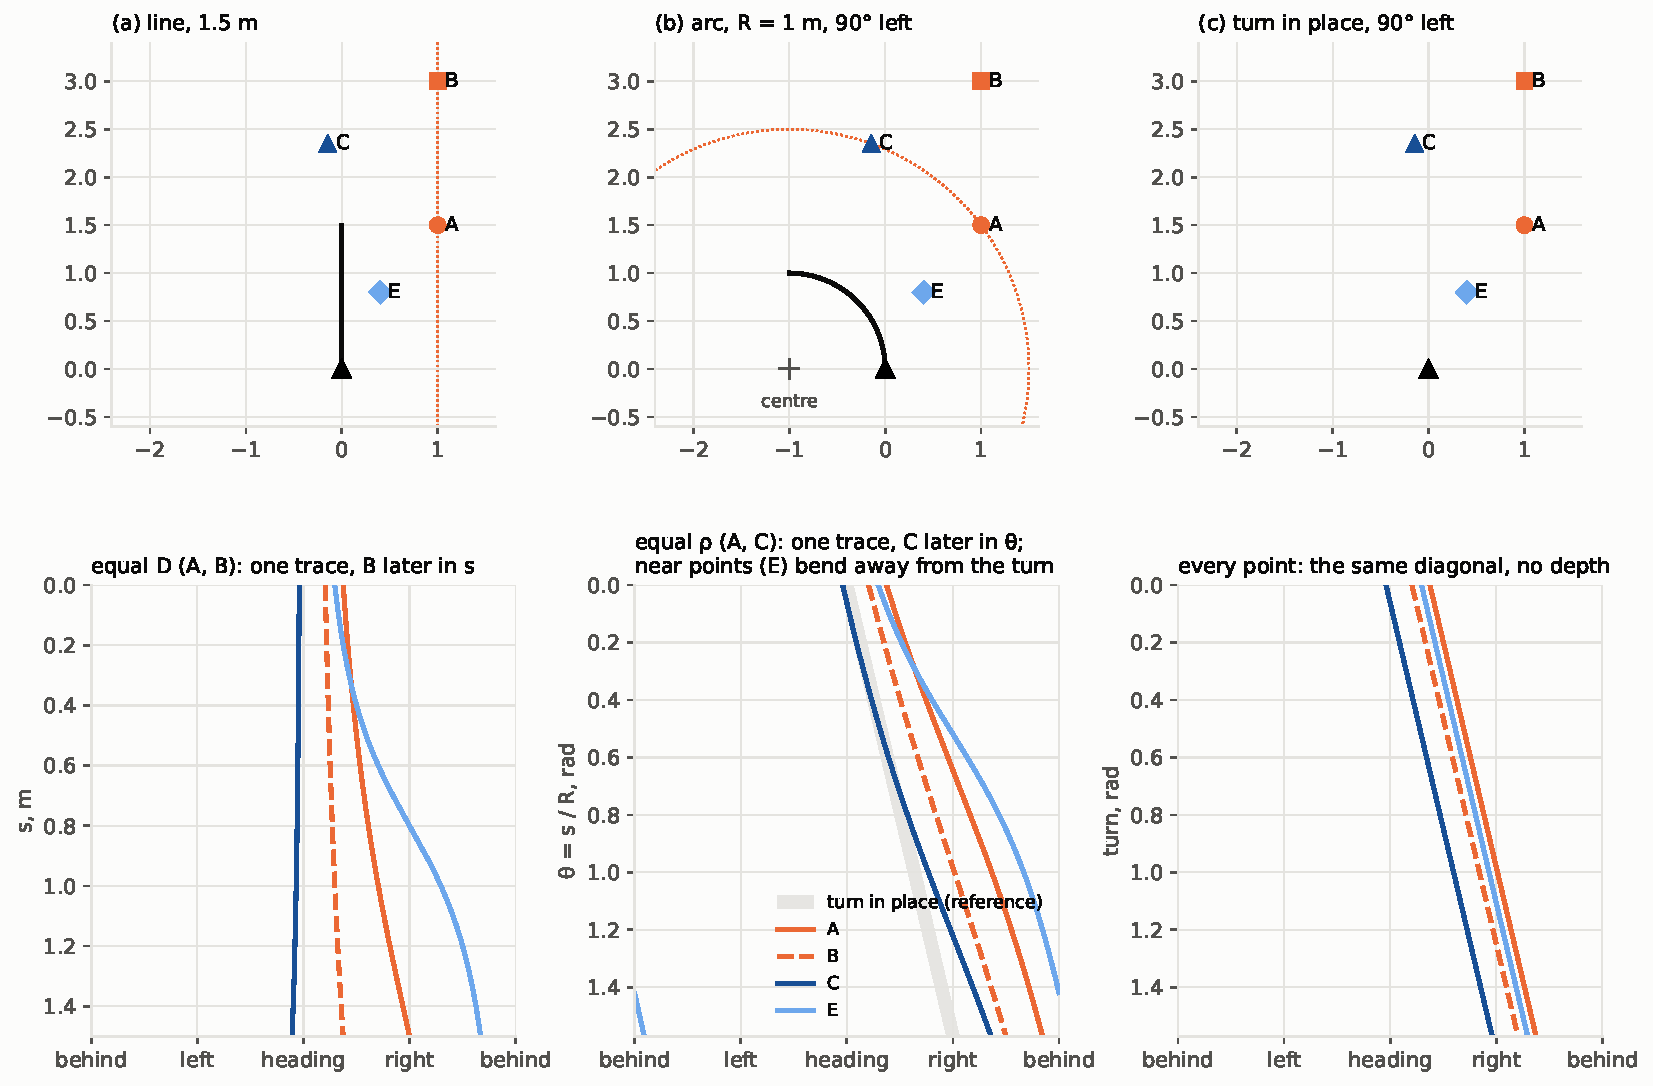
\includegraphics[width=\linewidth]{traces_primitives.pdf}
\caption{The same four points under a line (a), an arc of radius 1\,m turning $90^\circ$ left (b), and a turn in place
(c): top views (dotted: points of equal $D$ on the line, equal $\rho$ on the arc) and bearing against progress. On the arc,
the grey band is the turn in place; depth is a trace's departure from it. Formulas only.}\label{fig:traces-primitives}
\end{figure}

\begin{figure}[t]
\centering
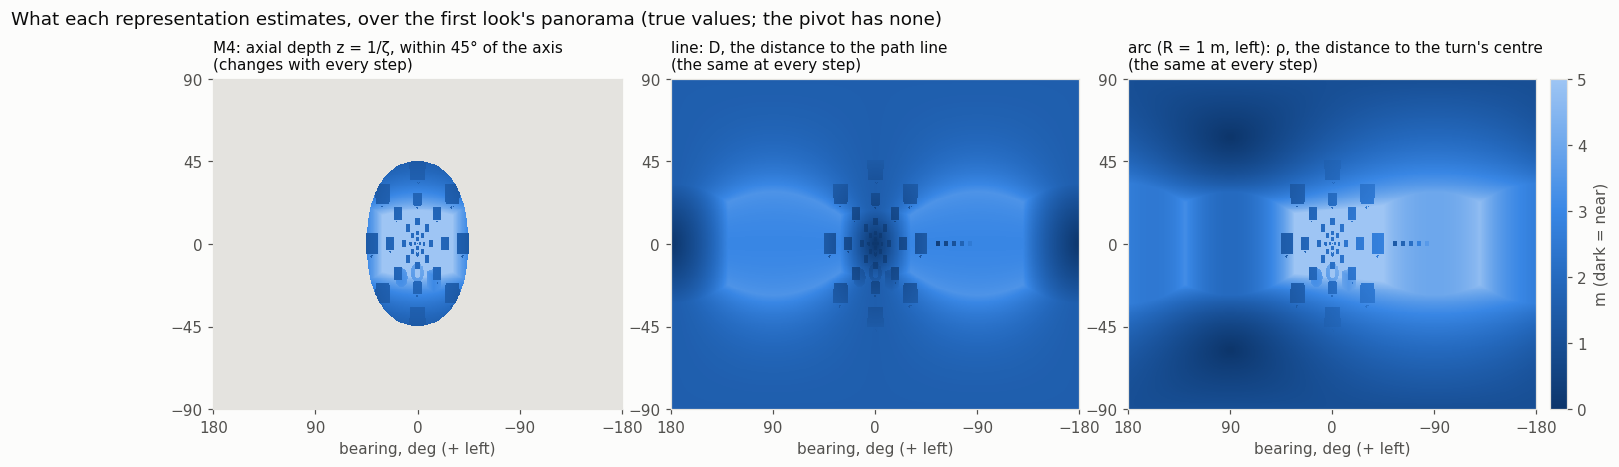
\includegraphics[width=\linewidth]{compare_invariants.png}
\caption{What each representation estimates, over a panorama of the calibration room (true values): M4's axial depth
$z$, within $45^\circ$ of the axis and for the current position only; the line's $D$; the arc's $\rho$ ($R=1$\,m, left).
The pivot has none. From \code{deep/compare.py}.}\label{fig:invariants}
\end{figure}

% ================================================================================================
\section{On the Riemann sphere}\label{sec:moebius}

Project the viewing sphere stereographically, with the FOE at $z=0$ and its opposite at $z=\infty$, and write
$\ell=\ln|z|=\ln\tan(\psi/2)$. M\"obius transformations, $z\mapsto(az+b)/(cz+d)$, are the conformal maps of this sphere;
they preserve the cross-ratio of any four points~\cite{needham}.

\paragraph{Rotations are M\"obius maps.} The rotations of the eye form the unitary part of $PSL(2,\mathbb C)$, so a turn
of the eye moves every direction by a M\"obius map, independently of depth. A turn in place about the vertical is an
\emph{elliptic} flow. This is why the pivot carries no depth.

\paragraph{Translation follows the hyperbolic maps.} The \emph{hyperbolic} M\"obius maps that fix the FOE and its opposite,
$z\mapsto kz$ with $k>0$, move every point along a meridian (a great circle through both foci: exactly the line's planes
$\omega=\text{const}$) by the same shift in $\ell$. A translation of the eye at unit speed moves a point at range $r$ along
the same meridian, at
\begin{equation}\label{eq:dl}
  \frac{d\ell}{dt} = \frac{1}{r}.
\end{equation}
Translation is therefore not a M\"obius map: it is the hyperbolic generator weighted, point by point, by inverse range.
Depth is exactly what breaks the M\"obius structure, and that is what we measure.

\paragraph{The line's coordinate.} With $\tau=\tan(\psi/2)=e^{\ell}$, $\cot\psi=(1-\tau^2)/(2\tau)$, so
\begin{equation}\label{eq:sinh}
  u=\cot\psi=-\sinh\ell .
\end{equation}
A hyperbolic M\"obius map shifts $\ell$; a finite translation shifts $\sinh\ell$ by $t/D$, which is
equation~\eqref{eq:line}. M4's coordinate is $q=\ln\tan\psi\approx\ell+\ln2$ near the FOE, which is why it behaved as a
pure shift in the fovea and less so towards $45^\circ$.

\paragraph{The arc is the sum.} At each instant, an arc's image motion is the turn's elliptic field (about the vertical,
depth-free) plus the translation's $1/r$-weighted hyperbolic field (about the tangent). Depth on an arc is the
departure of a trace from the turn-in-place diagonal (Figures~\ref{fig:traces-primitives}b and~\ref{fig:sphere}d).

\paragraph{Checks.} Four statements, each with a control that must fail, pass in \code{deep/moebius.py}\SB: (M1)
equation~\eqref{eq:dl} for random directions and ranges, to $7.6\times10^{-7}$ relative (the unweighted field is off by up
to 139\,\%); (M2) equation~\eqref{eq:sinh} and the finite shift of $\sinh\ell$ by $t/D$, to $1.3\times10^{-11}$ (one shift
of $\ell$ for all points is off by 0.92); (M3) a rotation preserves the cross-ratio of any four directions to below
$10^{-14}$, while every translation tried changed it by at least $1.8\times10^{-3}$; (M4) the arc's image motion equals the
elliptic plus weighted hyperbolic fields to $4.1\times10^{-6}$ (without the elliptic part, the median error is 0.85\,rad per
metre).

\paragraph{Why the name.} The method works with finite \emph{traces}, whole trajectories predicted by one number over a
piece of path, not with instantaneous flow; and their geometry is that of M\"obius transformations and their
depth-weighted relatives. Two echoes deserve a literature check: $PSL(2,\mathbb C)$ is also the Lorentz group acting on the
celestial sphere, where a boost is a hyperbolic M\"obius map (aberration~\cite{penrose}); and log-polar coordinates
$w=\log z$ turn the hyperbolic and elliptic maps about one pair of fixed points into translations, the usual reading of
the retino-cortical log-polar map~\cite{schwartz} that started this series.

\begin{figure}[t]
\centering
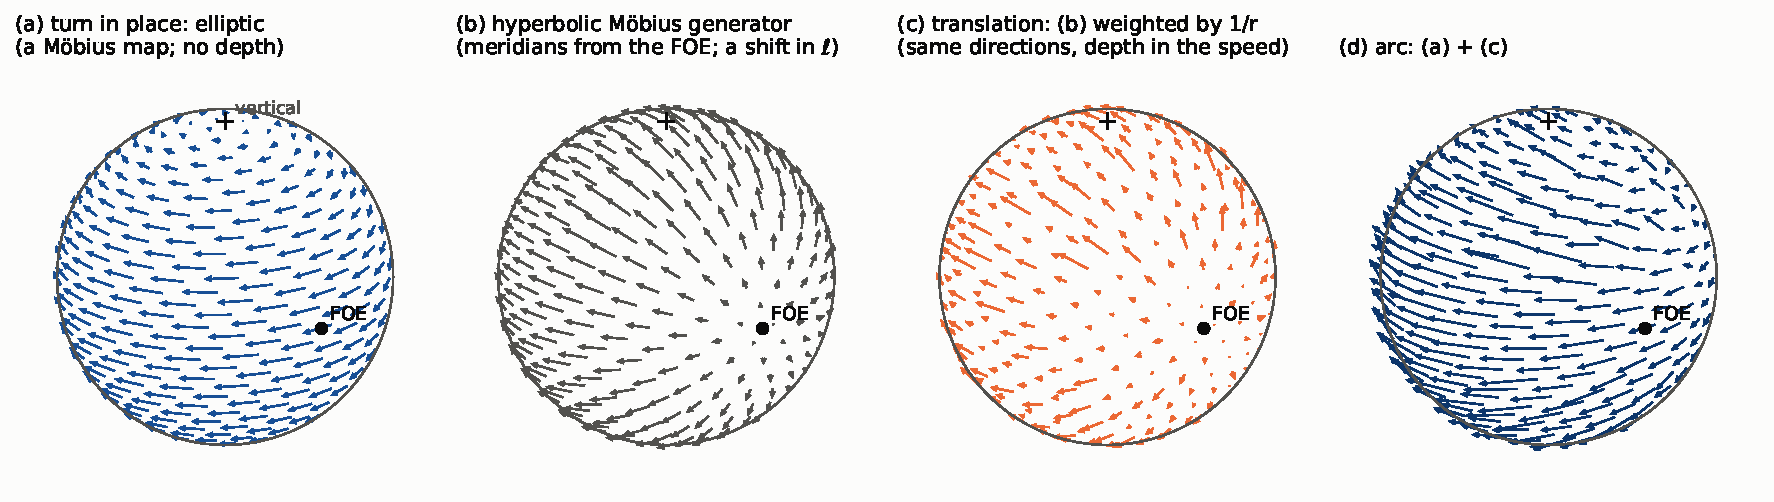
\includegraphics[width=\linewidth]{sphere_fields.pdf}
\caption{Image motion on the viewing sphere. (a) A turn in place: an elliptic M\"obius flow about the vertical, the same
at every depth. (b) The hyperbolic M\"obius generator: meridians from the FOE, a uniform shift in $\ell$. (c) A translation:
the field of (b) weighted by $1/r$ (ranges drawn at random between 0.8 and 5\,m); the directions are the same, the speeds
carry depth. (d) An arc: (a) plus (c). Formulas only.}\label{fig:sphere}
\end{figure}

% ================================================================================================
\section{Two ways to cut the space-time volume}\label{sec:mosaics}

Stack a sensor's images along the path and the result is a volume: direction by time. A \emph{trace} follows one point
through it. A \emph{slit-scan mosaic} does the opposite: it fixes one direction in the head, a slit, and records what crosses
it over time. Figure~\ref{fig:mosaics} shows mosaics from four slits under the three primitives.

On a line, the side slits record push-broom images of the walls, while the heading slit records only streaks: points
slide along it and never cross it. That is the line's blind direction, made visible. Under a turn in place every slit
records the same panorama, shifted in time by the slit's bearing: nothing depends on distance. On an arc there are no
streaks: points cross every slit, including the one dead ahead.

Comparing two mosaics turns depth into a time offset (Figure~\ref{fig:pairs}). On the arc, a point crosses the radial
slit (pointing through the turn's centre) when the eye, the centre and the point line up, a moment that does not depend on
its distance; it crosses any other slit at a time that does. For the slits at $-90^\circ$ and $-60^\circ$ the offset is
$\arccos(R\cos\beta/\rho)-60^\circ$, which tends to the $30^\circ$ between the slits as $\rho$ grows: a far point behaves as
in a turn in place, and its parallax, the shortfall from $30^\circ$, falls as $1/\rho$. On the line the offset grows in
proportion to $D$: $\Delta s=D\cot60^\circ$. Every crossing point in the calibration room falls on its curve\SB.

The two cuts are the same data. Matching along traces checks a predicted trajectory; matching mosaics is stereo between
two slit images, with the offset converted to $\rho$ or $D$ by a known one-dimensional function. The mosaic form is the more
intuitive, but near points also shift in elevation between slits (the vertical distortion known from concentric mosaics),
so its search is not strictly along a row; one guess of the invariant predicts both the time and the elevation of a trace.

\begin{figure}[t]
\centering
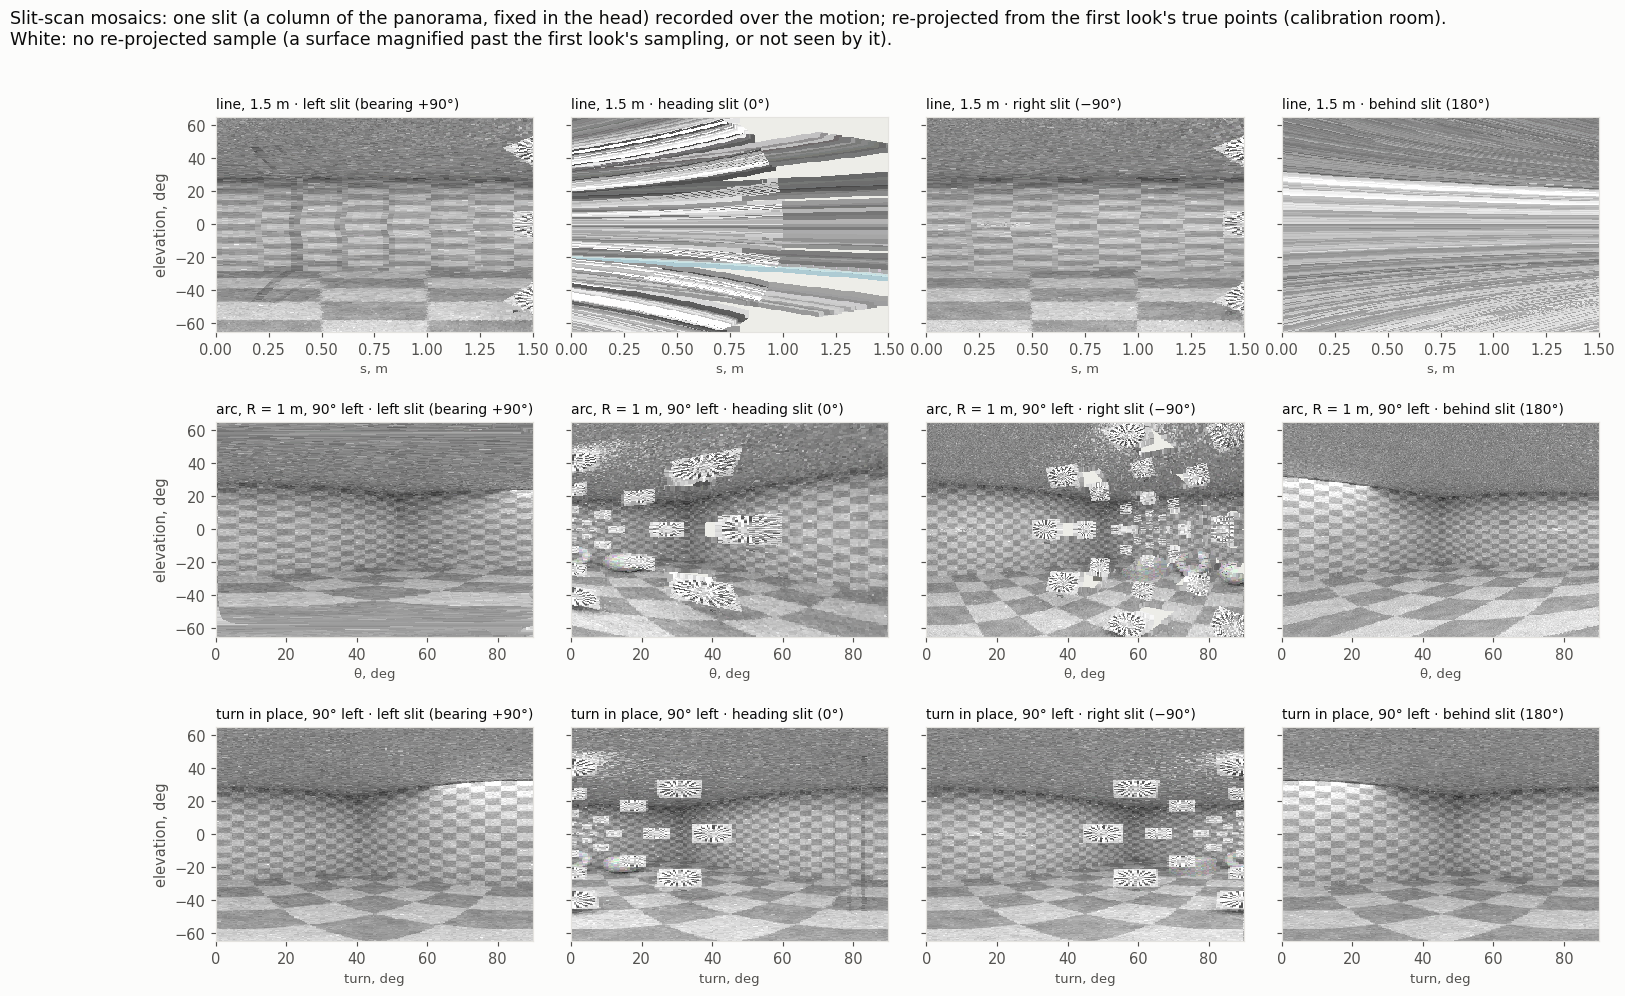
\includegraphics[width=\linewidth]{compare_mosaics.png}
\caption{Slit-scan mosaics in the calibration room: rows are the motions (a 1.5\,m line, an arc of radius 1\,m turning
$90^\circ$, a $90^\circ$ turn in place), columns are four slits fixed in the head (left, heading, right, behind). Each panel
is one column of the panorama recorded over the motion. Re-projected from the first look's true points (white: no sample).
From \code{deep/compare.py}\SB.}\label{fig:mosaics}
\end{figure}

\begin{figure}[t]
\centering
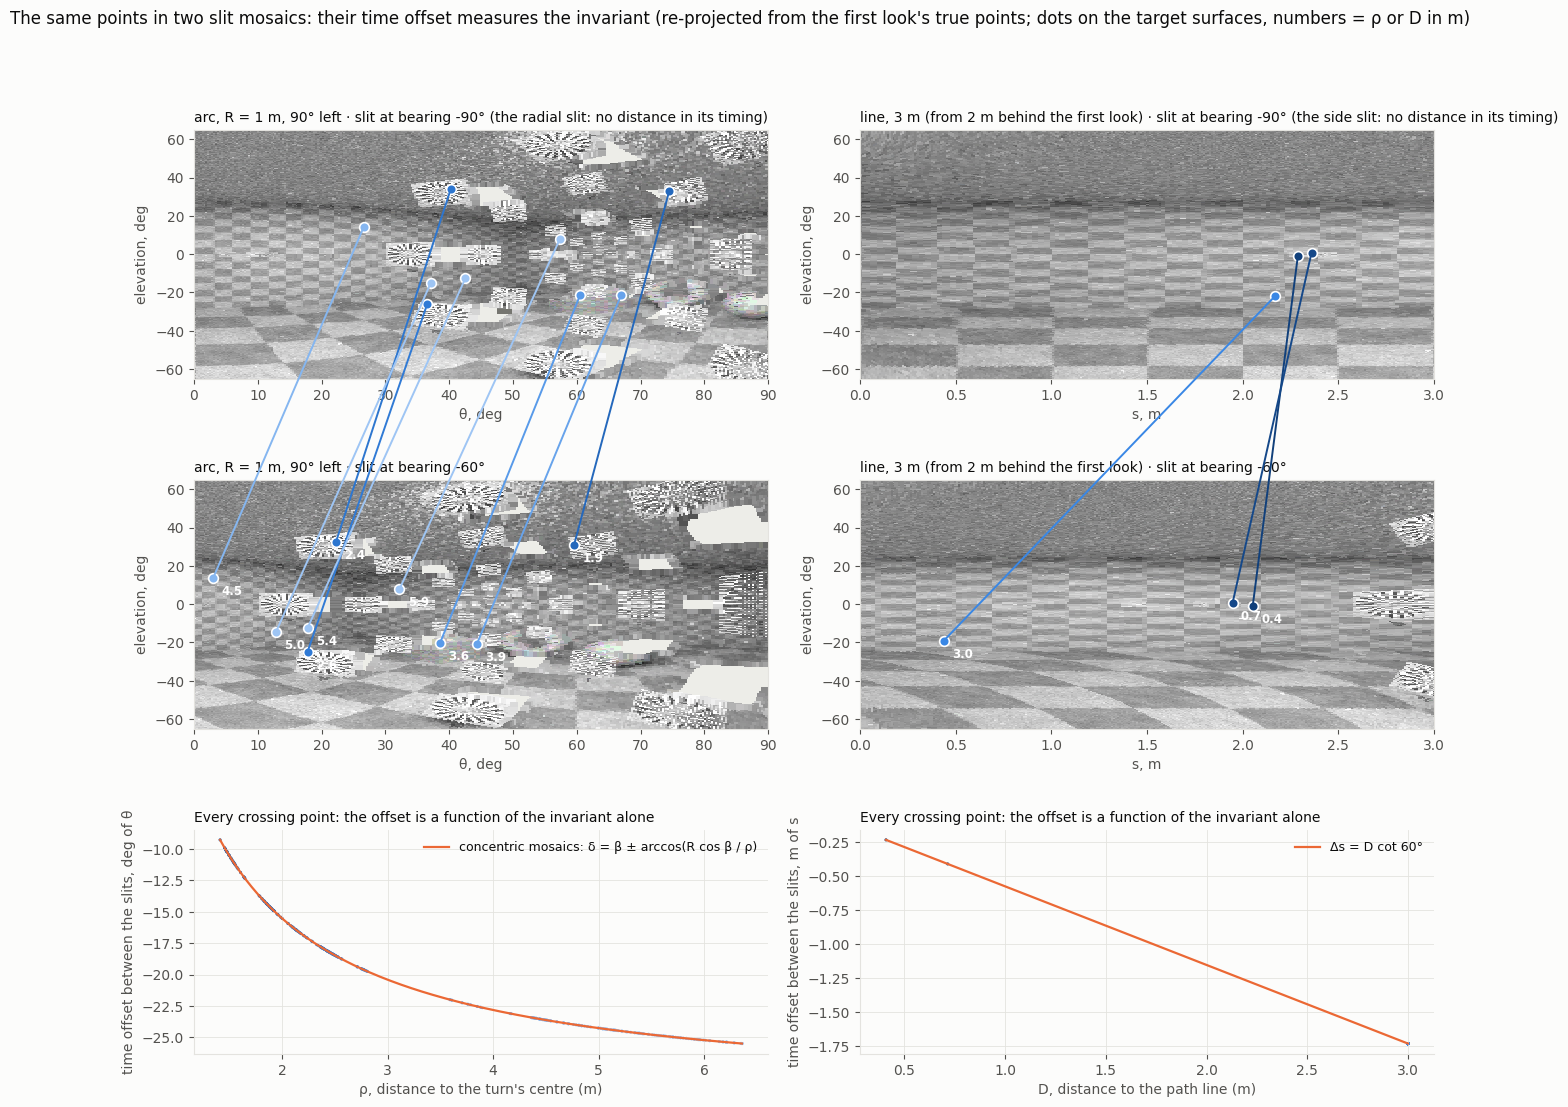
\includegraphics[width=0.92\linewidth]{compare_pairs.png}
\caption{The same points in two slit mosaics, linked. Left: the arc, the radial slit ($-90^\circ$) above a slit $30^\circ$
ahead of it. Right: a 3\,m line, the side slit above a slit $30^\circ$ ahead. Bottom: the time offset against $\rho$ or $D$
for every point that crosses both slits, on the predicted curves. Re-projected, as Figure~\ref{fig:mosaics}\SB.}\label{fig:pairs}
\end{figure}

% ================================================================================================
\section{Where depth is precise, and how often to look}\label{sec:atlas}

Before rendering anything, a Fisher model gives the precision of range along each direction: an anchor ray, its bearing
measured every 1\,cm over a 1\,m window with $0.1^\circ$ noise, known poses (Figure~\ref{fig:atlas}; a design model, not a
measurement). Table~\ref{tab:atlas} gives the relative standard deviation at 3\,m\SB.

\begin{table}[h]
\centering\small
\begin{tabular}{@{}lcccccc@{}}
\toprule
bearing from the heading & $1^\circ$ & $10^\circ$ & $30^\circ$ & $90^\circ$ & $150^\circ$ & $179^\circ$\\
\midrule
line & 0.097 & 0.0097 & 0.0035 & 0.0019 & 0.0035 & 0.097\\
arc, $R=4$\,m & 0.038 & 0.011 & 0.0036 & 0.0018 & 0.0036 & 0.038\\
arc, $R=1.6$\,m & 0.015 & 0.011 & 0.0037 & 0.0018 & 0.0037 & 0.015\\
\bottomrule
\end{tabular}
\caption{$\sigma_r/r$ at 3\,m (1\,m window, 1\,cm steps, $0.1^\circ$). Exactly on the heading the line is blind; the arcs give
0.034 and 0.014.}\label{tab:atlas}
\end{table}

Arcs have no blind direction: curving the path fills the line's blind cone, more so for tighter turns. Elsewhere lines and
arcs agree within about 10\,\% (at $10^\circ$ from the heading the arcs are slightly worse), and the lateral directions are
the most precise on both. A check declared beforehand that the arc's turn axis carries no range \emph{failed}
(information 1.28): that is how the absence of a blind direction was found\SB.

The same model gives the time step. Before a point's range is known (a prior band of 0.5--20\,m), a lateral ray needs steps
under 1\,mm to stay within one resolution element; once range is within $\pm10$\,\%, 2.6\,cm suffices laterally and 30\,cm
near the heading\SB. Sampling in time should be driven by uncertainty: fine while uncertain, coarse once converged, per
direction and per point.

\begin{figure}[t]
\centering
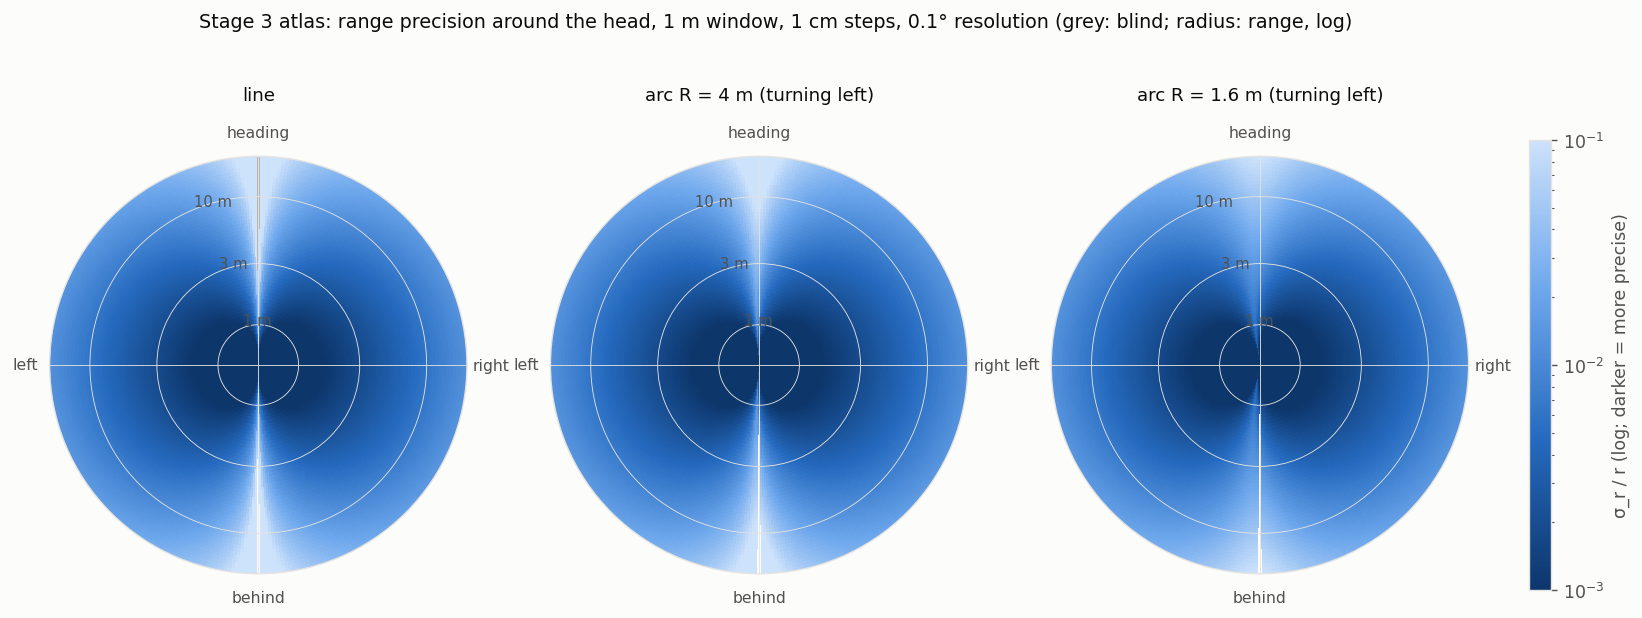
\includegraphics[width=\linewidth]{stage3_atlas.png}
\caption{The information atlas: precision of range around the head for a line and two arcs (1\,m window, 1\,cm steps,
$0.1^\circ$; radius is range, logarithmic). The line is blind along its path line; the arcs are not. From
\code{deep/atlas.py}\SB.}\label{fig:atlas}
\end{figure}

% ================================================================================================
\section{The sensor}\label{sec:sensor}

Any sensor that does the job is acceptable: in a synthetic world a sensor is a choice of rays. The design is a fan of
vertical slits locked to the heading. It is carried by fov-render's~\cite{fovrender} equirectangular Panorama sensor,
which needs no change: with the head locked to the tangent, each column is a slit at a bearing and each row an elevation,
which are exactly the arc's concentric-mosaic coordinates; the line's coordinates come from the same rays
(Figure~\ref{fig:slitfan}). Per-slit time sampling is emulated by keeping each column's samples at its own rate. A first
check caught the first-order time step overshooting a pixel by 5.5\,\% for a near point at $10^\circ$ from travel; the
schedule is now solved exactly, by bisection\SB. In the sandbox a look of $720\times360$ (0.5$^\circ$ per pixel) takes about
10\,s at 16 samples per pixel\SB; at the design resolution, $3600\times1800$ ($0.1^\circ$), about 12--15\,s on the GPU, most of
it writing the outputs\WS.

\begin{figure}[t]
\centering
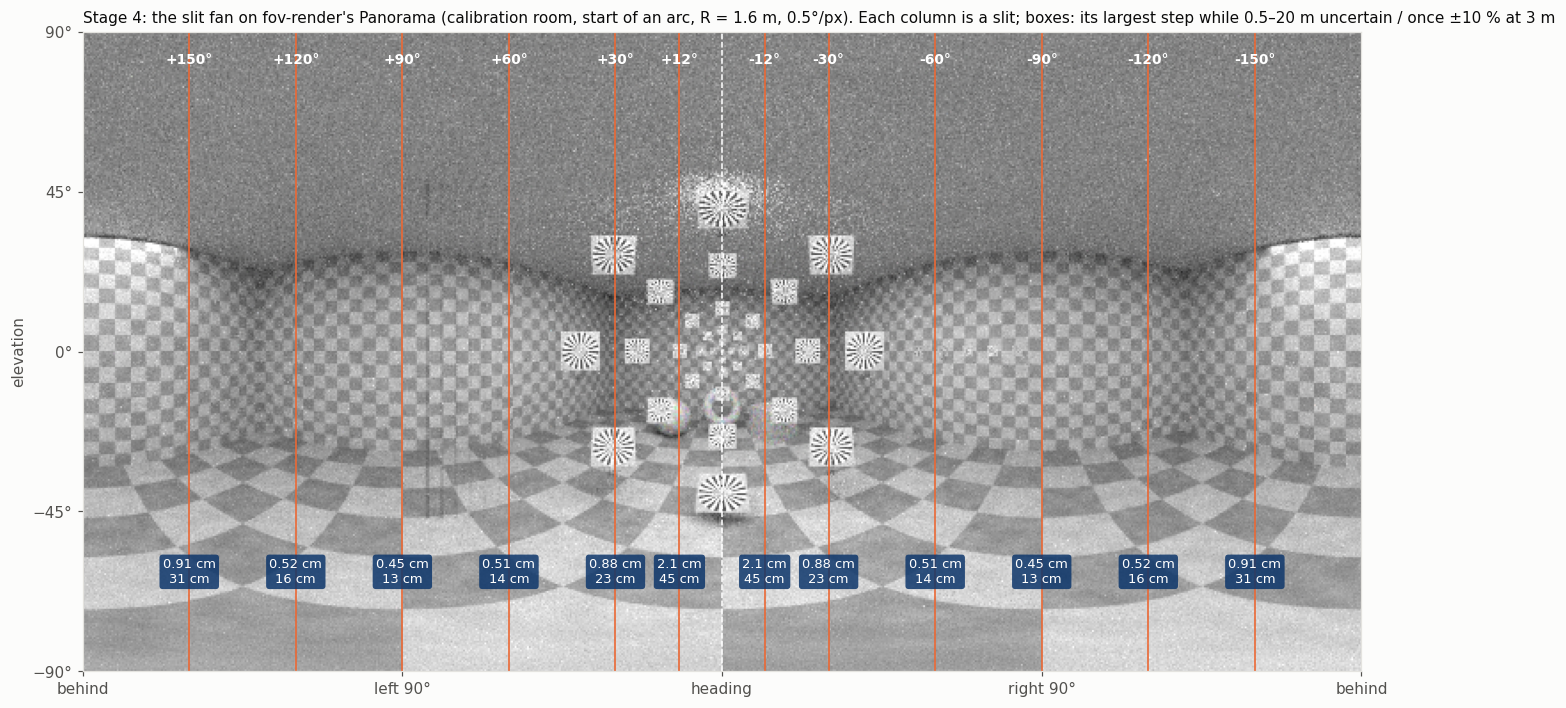
\includegraphics[width=\linewidth]{stage4_slit_fan.png}
\caption{The slit fan on fov-render's Panorama (calibration room, start of an arc, $R=1.6$\,m, $0.5^\circ$ per pixel). Each
column is a slit; the boxes give its largest time step while range is uncertain (0.5--20\,m) and once it is within
$\pm10$\,\% at 3\,m. From \code{deep/sensor.py}\SB.}\label{fig:slitfan}
\end{figure}

% ================================================================================================
\section{The oracle and the fusion}\label{sec:oracle}

The formulation is judged with an oracle first, as in the project's binocular work: each point's true position (from the
renderer) gives its true trace; bearing and elevation get Gaussian noise of 0.25, 0.5 or 1\,px; range along the ray is
fitted by Gauss--Newton through the known poses. A range is \emph{usable} when its 95\,\% interval is within $\pm10$\,\%.

\paragraph{Short windows (stage 5a, sandbox).} On renders of the calibration room the oracle recovers range exactly without
noise ($1.4\times10^{-13}$), its precision equals the atlas's to $10^{-4}$, the pivot carries no range, and its intervals cover
the truth 94.9--95.0\,\% of the time\SB. At $0.5^\circ$ per pixel the arc's gain at the heading is real but small: with 50\,cm
windows, $\pm44$\,\% against the line's $\pm114$\,\% in the $2^\circ$ cone, with the wall 4.8\,m ahead\SB.

\paragraph{Long windows (stage 5b.1, workstation).} At the design resolution ($0.1^\circ$) with 1\,m windows, the arc makes
the heading usable: in the $2^\circ$ cone, $\pm1.1$\,\% against $\pm4.6$\,\% on the line, at 4.7\,m, and usable at every
noise level where the line's fraction falls from 94 to 60 to 2\,\%\WS (Figure~\ref{fig:profile}). The sandbox's atlas
predicted $\pm1.10$--$1.14$\,\%\SB.

\begin{figure}[t]
\centering
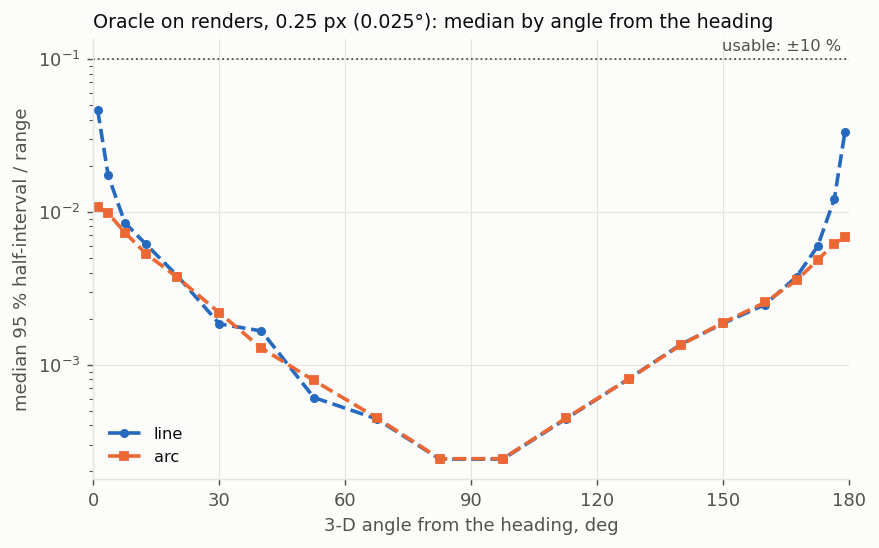
\includegraphics[width=0.72\linewidth]{stage5b1_profile.png}
\caption{Oracle on renders at the design resolution: median 95\,\% half-interval of range against the angle from the heading,
for a 1\,m line and a 1\,m arc ($R=1.6$\,m) at 0.25\,px. The arc closes the line's cone at the heading and behind. Code,
workstation\WS.}\label{fig:profile}
\end{figure}

\paragraph{Fusion in world 3D (stage 5b.2).} Neighbouring windows share looks, so merging their estimates would count each
measurement several times. The oracle's fusion is instead a joint fit: each 2\,cm surface cell is fitted to its bearing and
elevation in every look that sees it, each look once, with the Fisher covariance as its uncertainty. The check that this
uncertainty is honest gives a standard deviation of normalised errors of 0.9993; counting each look twice, which is what
merging overlapping windows does, gives 1.413\SB. One failure is worth recording: on the workstation's 90$^\circ$ turn, one
cell of 199{,}991 under the arc stalled at a look's nadir, where the bearing is undefined (2.6\,\% of range). Code traced it;
the fit now starts from the least-squares intersection of the observed rays (or from the earlier start, if that fits
better), a new check (F1b) on 2{,}000 synthetic floor cells under the turn passes with its control (the earlier start)
failing, and no threshold moved\SB\WS.

Table~\ref{tab:fusion} compares a 90$^\circ$ turn (30\,cm line, arc of radius 1\,m, 30\,cm line; 2.17\,m) with a straight
path of the same length, 218 looks each at 1\,cm and $0.1^\circ$\WS. With perfect correspondences both saturate: about
99\,\% of the visible surface is usable at 0.5\,px in both scenes. Path geometry shows at the margins, and the margins
depend on the scene: in the calibration room the turn is complete sooner and has the smaller error tail; in the Classroom
the curves coincide and the straight path's tail is smaller. At the coarser sandbox resolution the turn's advantage is
clearer: 98.4 against 94.2\,\% usable, and 98.6 against 74.3\,\% in the cone ahead\SB.

\begin{table}[h]
\centering\small
\begin{tabular}{@{}llccc@{}}
\toprule
scene & path & usable, 0.25 / 0.5 / 1\,px & 3-D error, median / p95 & 95\,\% after\\
\midrule
calibration room & turn & 99.95 / 99.87 / 99.75\,\% & 1.1 / 7.4\,mm & 0.68\,m\\
 & straight & 99.87 / 99.71 / 99.36\,\% & 1.1 / 19.9\,mm & 0.87\,m\\
Classroom & turn & 99.71 / 99.23 / 98.33\,\% & 1.5 / 25.4\,mm & 1.35\,m\\
 & straight & 99.64 / 99.28 / 98.59\,\% & 1.4 / 21.6\,mm & 1.36\,m\\
\bottomrule
\end{tabular}
\caption{Fusion with the oracle at the design resolution (errors at 0.5\,px). In the Classroom the 95\,\% intervals cover the
truth 94.96--95.06\,\% of the time.
The two paths start 2\,m apart, so each sees its own surroundings. Code, workstation\WS.}\label{tab:fusion}
\end{table}

\paragraph{A tour.} The two Classroom paths join into one L-shaped tour: 2\,m up the aisle, then the $90^\circ$ arc, 4.17\,m
and 418 looks in all. A video shows the fusion growing look by look (Figure~\ref{fig:demo}); at the end 99.3\,\% of the
cells are usable, and the video's per-frame estimate equals the full fusion to $1.3\times10^{-4}$ of its standard
deviation\WS. It is the turn-in-place tour of the previous note~\cite{tr2}, with the turn made smooth.

\begin{figure}[t]
\centering
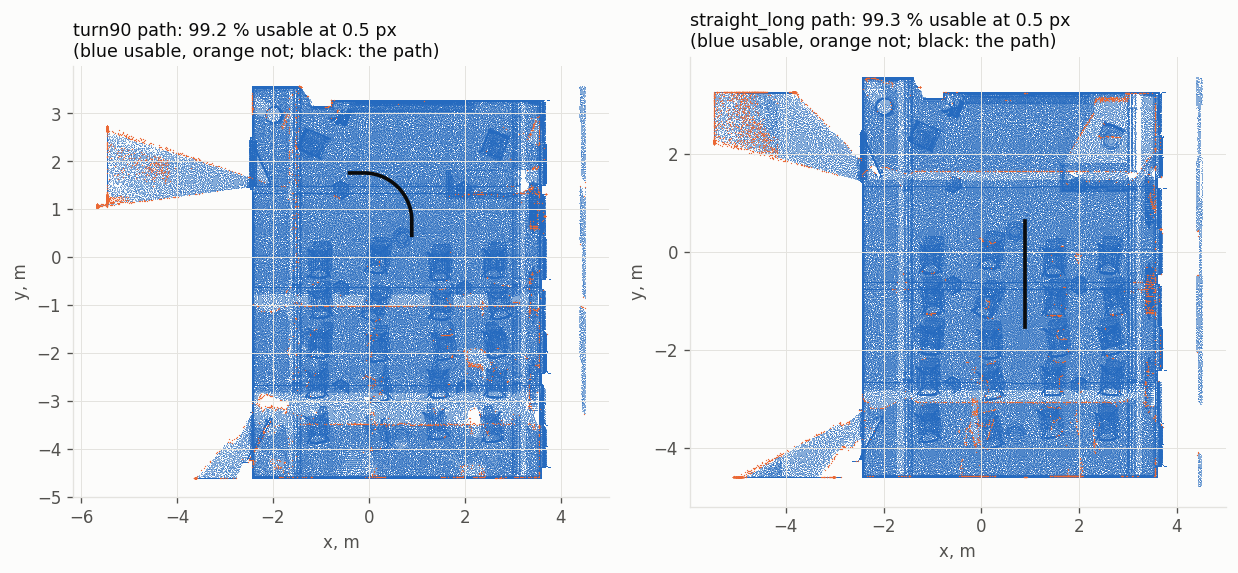
\includegraphics[width=\linewidth]{stage5b2_classroom_topdown.png}
\caption{The Classroom from above, fused with the oracle at 0.5\,px: the $90^\circ$ turn (left) and the straight path
(right). Blue usable, orange not; cells outside the room are seen through a door, an opening and the windows. Code,
workstation\WS.}\label{fig:classroom}
\end{figure}

\begin{figure}[t]
\centering
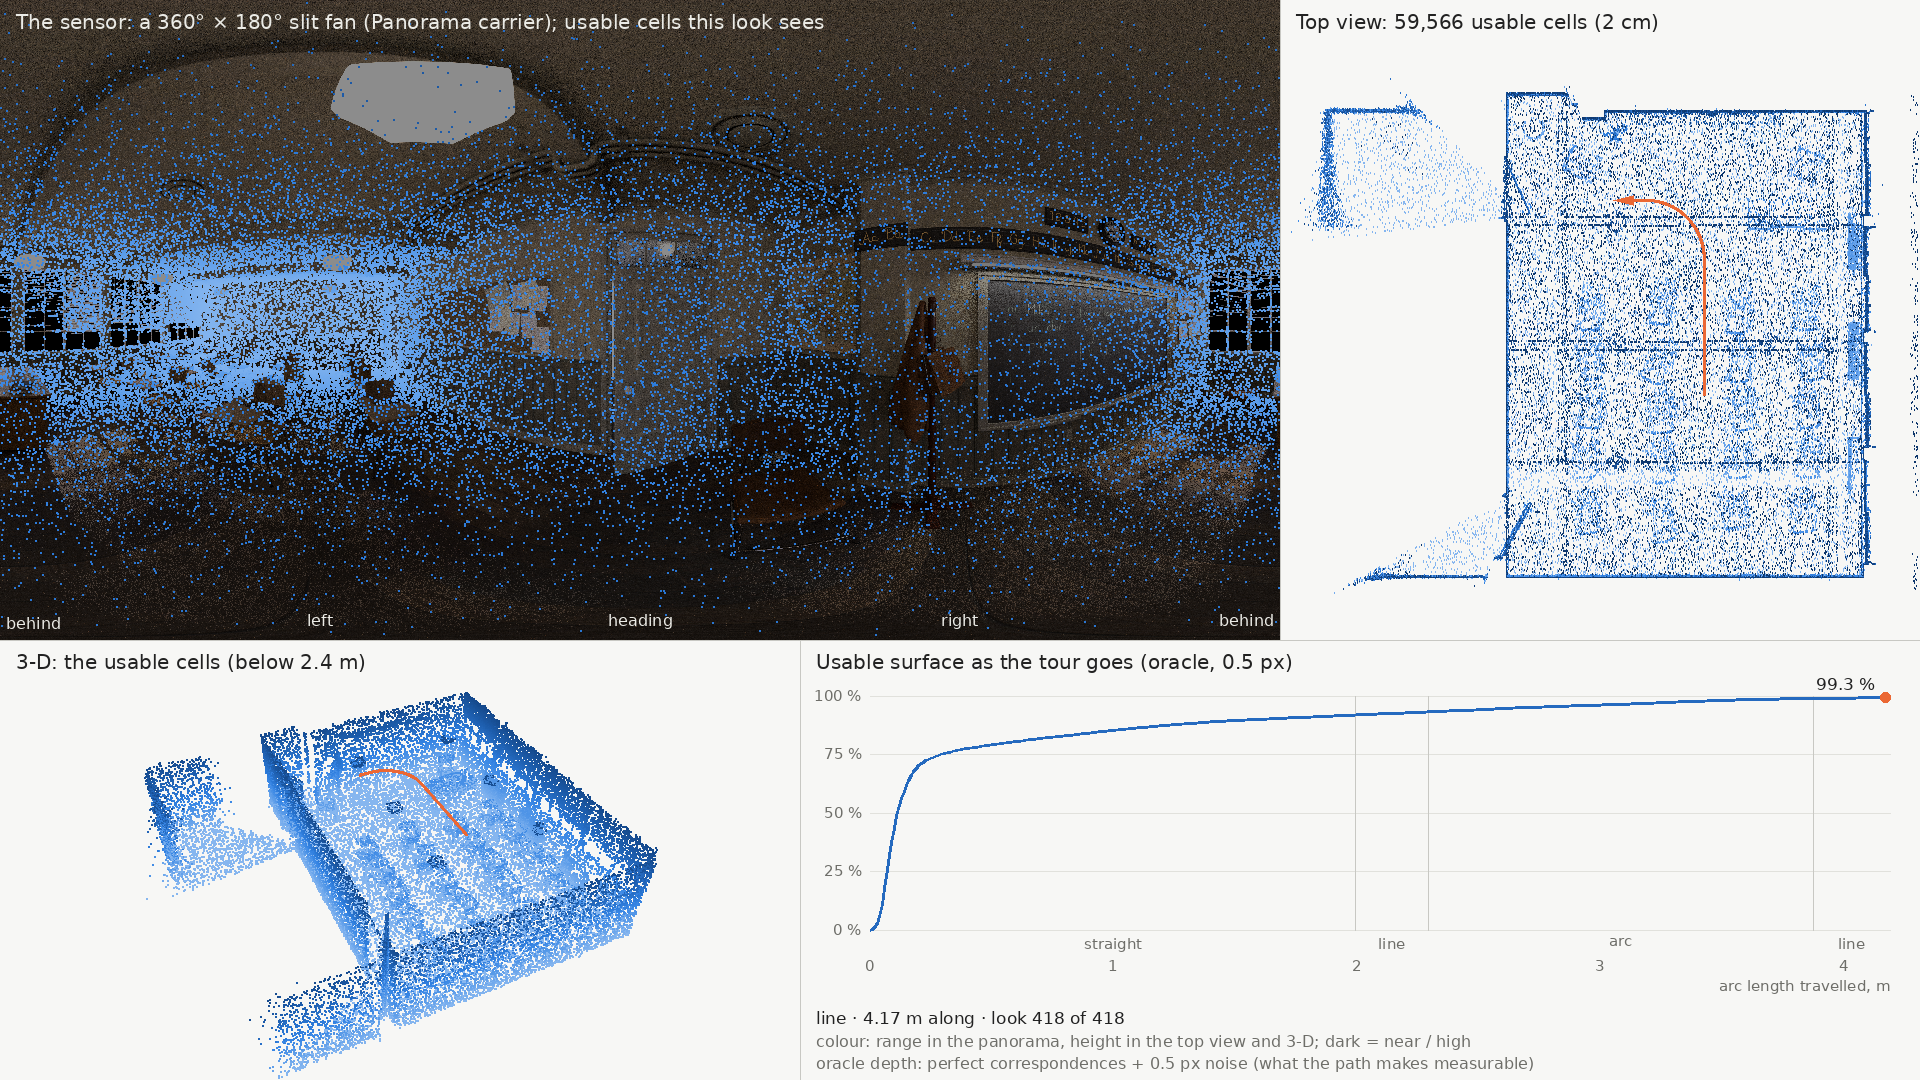
\includegraphics[width=\linewidth]{demo_last_range.png}
\caption{The last frame of the tour's video: the panorama with the usable cells it sees (coloured by range), the top view,
the 3-D cells below 2.4\,m, and the usable fraction along the tour. Oracle depth. Code, workstation\WS.}\label{fig:demo}
\end{figure}

\FloatBarrier
% ================================================================================================
\section{What remains}\label{sec:remains}

\paragraph{Real matching.} Everything above uses perfect correspondences. The formulation tells a matcher what to deliver:
at 1\,cm steps and $0.1^\circ$ pixels a point 2\,m to the side moves about 3 pixels between looks (an estimate), so following it from one
look to the next is easy and keeping it over a hundred looks is the difficulty; and one guess of $D$ or $\rho$ predicts the
whole trace, so matching can be a one-dimensional sweep over the invariant that scores how consistent the samples along
each predicted trace are, which generalises epipolar-plane-image analysis~\cite{bolles} from lines to arcs, or stereo
between slit mosaics. The failures will be photometric, not geometric: occlusion edges where traces end, textureless
surfaces, highlights, and the window band where rays hit nothing.

\paragraph{Instantaneous flow.} The method uses finite traces over a whole piece of path. Instantaneous optical flow is a
different and complementary view: equation~\eqref{eq:dl} says that, at each instant, the flow along a meridian measures
inverse range directly, and the decomposition into an elliptic (rotation) and a weighted hyperbolic (translation)
field~\cite{longuethiggins} holds at every moment, not only along a primitive. Flow could seed a trace's guess, track
points between looks, handle paths that are not yet split into primitives, or estimate the motion itself. What flow brings
to the picture, and how it should be combined with traces, is a question to explore.

\paragraph{Other open questions.} Sampling in time driven by uncertainty (Section~\ref{sec:atlas}); joints between pieces
(clothoids) and paths in 3D (helices); transitions between perceptual regimes (binocular, lateral sway, forward motion),
read as weighting by information rather than switching; the action policy that chooses the path; and a literature search on
concentric mosaics~\cite{shum}, stereo panoramas~\cite{peleg}, crossed-slits projections~\cite{zomet} and
epipolar-plane-image analysis~\cite{bolles} before any claim of novelty.

\paragraph{Limitations.} Synthetic images; known motion (the poses come from the path); the oracle stands in for matching;
two scenes; and a short arc ($10.7^\circ$) in the sandbox changed almost nothing overall, so a turn must be real to matter.

% ================================================================================================
\section{How the work was done}\label{sec:process}

The method is the N-Surface method~\cite{nsurface} in its light form: one file of rules and GitHub issues as the channel
between Claude in a chat sandbox (``Chat''), which planned, wrote the code and its checks and ran what a CPU can, and
Claude Code on the RTX~4090 workstation (``Code''), which rendered at the design resolution and ran the Classroom. Luiz
decided: the reformulation after a brainstorm he asked to keep open until it closed by itself, the primitives, the
oracle-first order, the sensor's rendering path, the splits of stage 5, and the name. Every check shipped with a control
that must fail. Several checks failed on their first run, and three of those failures taught something about the
geometry (the arc's missing blind direction, the first-order time step, the stall at a nadir); none had its threshold
moved. The work in this note took four days, 16 to 19 November 2026.

\paragraph{Records.} Everything above is in \code{visgraf/deep-motion}~\cite{dm}: \code{docs/plan.md} (the plan, the
decisions P-D1 to P-D3, and every result with its command and commit), \code{docs/runs/issue-2/} to \code{issue-11/}, and
issues \#2 to \#11. The demo's videos stay on the workstation. Figure sources are listed in \code{figs/SOURCES.md}.

% ================================================================================================
\begin{thebibliography}{99}
\bibitem{dm} VISGRAF Lab. \emph{deep-motion}: depth from motion along curved paths.
  \url{https://github.com/visgraf/deep-motion}
\bibitem{tr2} Luiz Velho and Claude. ``Foveated Vision on a Moving Head: Depth from Forward Motion''. VISGRAF technical
  note, 15 November 2026. \url{https://github.com/lvelho/foveal-depth-tr}
\bibitem{fovrender} VISGRAF Lab. \emph{fov-render}: Blender Cycles rendering for gaze-directed binocular observers.
  \url{https://github.com/visgraf/fov-render}
\bibitem{nsurface} Luiz Velho and Claude. ``The N-Surface Method: Rigor and Spontaneity in Human--AI Research''.
  VISGRAF technical note, 2026.
\bibitem{okutomi} M.~Okutomi and T.~Kanade. A multiple-baseline stereo. \emph{IEEE Transactions on Pattern Analysis and
  Machine Intelligence}, 15(4):353--363, 1993.
\bibitem{bolles} R.~C. Bolles, H.~H. Baker and D.~H. Marimont. Epipolar-plane image analysis: an approach to determining
  structure from motion. \emph{International Journal of Computer Vision}, 1(1):7--55, 1987.
\bibitem{shum} H.-Y. Shum and L.-W. He. Rendering with concentric mosaics. In \emph{Proceedings of SIGGRAPH~99}, pages
  299--306, 1999.
\bibitem{peleg} S.~Peleg and M.~Ben-Ezra. Stereo panorama with a single camera. In \emph{Proceedings of the IEEE Conference
  on Computer Vision and Pattern Recognition}, pages 395--401, 1999.
\bibitem{zomet} A.~Zomet, D.~Feldman, S.~Peleg and D.~Weinshall. Mosaicing new views: the crossed-slits projection.
  \emph{IEEE Transactions on Pattern Analysis and Machine Intelligence}, 25(6):741--754, 2003.
\bibitem{longuethiggins} H.~C. Longuet-Higgins and K.~Prazdny. The interpretation of a moving retinal image.
  \emph{Proceedings of the Royal Society of London B}, 208:385--397, 1980.
\bibitem{needham} T.~Needham. \emph{Visual Complex Analysis}. Oxford University Press, 1997.
\bibitem{penrose} R.~Penrose. The apparent shape of a relativistically moving sphere. \emph{Proceedings of the Cambridge
  Philosophical Society}, 55:137--139, 1959.
\bibitem{schwartz} E.~L. Schwartz. Spatial mapping in the primate sensory projection: analytic structure and relevance
  to perception. \emph{Biological Cybernetics}, 25:181--194, 1977.
\end{thebibliography}

\end{document}
